\documentclass[10pt,xcolor={dvipsnames}]{beamer}

\usetheme[numbering=none]{metropolis}
\setbeamertemplate{note page}[plain]
\setbeameroption{show notes on second screen=right}

\usepackage[style=numeric]{biblatex}
\bibliography{TechTalkDotNetMemoryLeak}

\usepackage{graphicx}
\graphicspath{{../Presentation}}

\usepackage{listings}
\newsavebox\stackheapbox

\usetikzlibrary{arrows.meta}
\usetikzlibrary{overlay-beamer-styles}

\tikzset{
  file/.pic={
    \draw (0,0) -- (0,0.8) -- (0.45,0.8) -- (0.6,0.65) -- (0.6,0) -- (0,0);
    \draw (0.45,0.8) -- (0.45,0.65) -- (0.6,0.65);
  }}
\tikzset{
  dllfile/.pic={
    \draw (0,0) pic {file};
    \node [align=center] at (0.3,0.4) {\texttt{\scriptsize.dll}};
  }}
\tikzset{
  csfile/.pic={
    \draw (0,0) pic {file};
    \node [align=center] at (0.3,0.4) {\texttt{\scriptsize.cs}};
  }}
\tikzset{
  asm/.pic={
    \draw (0,0) rectangle (0.6,0.6);
    \node [align=center] at (0.3,0.3) {\texttt{\scriptsize ASM}};
  }}

\definecolor{light-grey}{gray}{0.9}

\title{Case study: debugging memory leaks in .NET}
\date{}

\begin{document}

\begin{frame}
  \titlepage
\end{frame}
\note[itemize]
{
  \item This tech talk is a case study of a memory leak in \texttt{CodeRunner}.
  \item It's quite gentle and reviews the fundamentals of .NET and memory management.
  \item We'll cover a small amount of theory interspersed with a simple example and the \texttt{CodeRunner} `bug'.
}

\begin{frame}[fragile]{Case study}
  \begin{center}
    \includegraphics[scale=0.3]{RamUsage.jpg}
  \end{center}
\end{frame}
\note[itemize]
{
  \item The bug report said that in a recent build of \texttt{CodeRunner} memory usage had significantly increased and resulted in the RAM on the VM being maxed.
  \item As can be seen in the \texttt{Task Manager} window some instances were using up to 3 GB.
  \item Normally the first step might be to see what changes have been made inbetween the last release and this release, but it didn't seem obvious (although it is in retrospect).
  \item With memory leaks there's two questions we might ask: where is the leak, and why is it leaking?
  \item This tech talk is divided into two parts to look at each question. Let's start with where\ldots
}

\section{Where?}
\note[itemize]
{
  \item We'll first review how memory management works in .NET.
  \item Then we'll look at a simple example that allocates memory.
  \item Finally we'll find out where the memory leak is in \texttt{CodeRunner}.
}

\begin{lrbox}{\stackheapbox}
\lstset{
  basicstyle=\ttfamily\small,
  columns=fullflexible,
  keepspaces=true,
}
\begin{lstlisting}
Allocate();

void Allocate()
{
  char stack;
  char[] heap = new char[1];
}
\end{lstlisting}
\end{lrbox}

\begin{frame}[fragile]{Stack \& heap}
  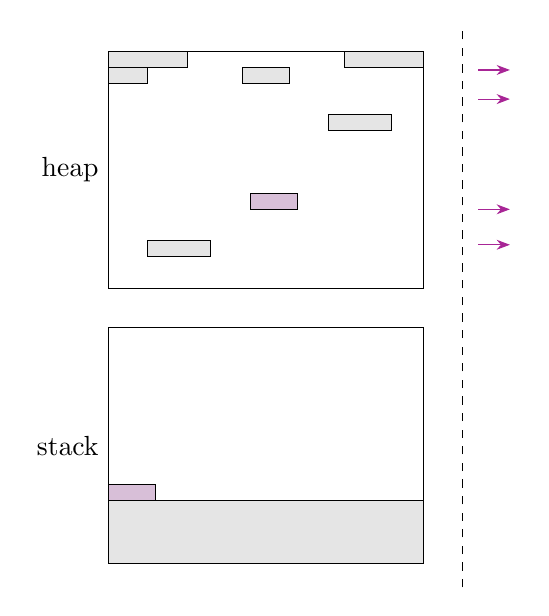
\begin{tikzpicture}[ampersand replacement=\&]
    % Heap
    \node [left] at (0,5) {heap};
    \draw (0,3.5) rectangle (4,6.5);
    \draw [fill=light-grey] (0,6.5) rectangle (1,6.3);
    \draw [fill=light-grey] (3,6.5) rectangle (4,6.3);
    \draw [fill=light-grey] (0,6.3) rectangle (0.5,6.1);
    \draw [fill=light-grey] (1.7,6.3) rectangle (2.3,6.1);
    \draw [fill=light-grey] (2.8,5.7) rectangle (3.6,5.5);
    \draw [fill=light-grey] (0.5,4.1) rectangle (1.3,3.9);
    \visible<3-4>{\draw [fill=Thistle] (1.8,4.5) rectangle (2.4,4.7);}
    % Stack
    \node [left] at (0,1.5) {stack};
    \draw (0,0) rectangle (4,3);
    \draw [fill=light-grey] (0,0) rectangle (4,0.8);
    \visible<2-3>{\draw [fill=Thistle] (0,0.8) rectangle (0.6,1);}
    % Code
    \draw [dashed] (4.5,-0.3) -- (4.5,6.8);
    \node [right] at (5,5) {\usebox\stackheapbox};
    % Code arrows
    \visible<1>{\draw [draw=Mulberry,-{Stealth}] (4.7,6.27) -- (5.1,6.27);}
    \visible<2>{\draw [draw=Mulberry,-{Stealth}] (4.7,4.5) -- (5.1,4.5);}
    \visible<3>{\draw [draw=Mulberry,-{Stealth}] (4.7,4.05) -- (5.1,4.05);}
    \visible<4>{\draw [draw=Mulberry,-{Stealth}] (4.7,5.9) -- (5.1,5.9);}
  \end{tikzpicture}
  \note<1>[item]{It's first useful to review how memory is allocated and unallocated (`freed').}
  \note<1>[item]{We have two sections of memory: the stack and the heap. Here we have a snippet of a simple program where we are in the middle of execution. The grey boxes in the stack and the heap represent memory that's already been allocated.}
  \note<1>[item]{Let's follow memory allocation in execution of this snippet.}
  \note<2>[item]{The first statement is something your compiler will warn you about---a variable that is declared but not used. But this variable (unless optimised away) will use memory on the stack.}
  \note<2>[item]{In C\# variables can be either value types or reference types. Primitive types are value types. As we'll see shortly the main effect of value types is that the memory allocation is \emph{scoped}.}
  \note<2>[item]{Value types aren't always allocated on the stack, but in the context of a function call evaluation like this they are.}
  \note<2>[item]{The stack contains fixed memory allocations and like other stacks these allocations are ``last in first out'' (LIFO) so they are unallocated in the reverse order to their allocation.}
  \note<3>[item]{This next line contains an array. Arrays are reference types. Reference types are always allocated on the heap so are easier to define than value types.}
  \note<3>[item]{The key thing about reference types is that their memory allocation is not \emph{scoped}, so their lifetime is controlled by whether anybody is using them.}
  \note<4>[item]{We can see this affect when we return from the method call. Here the stack allocation has been automatically freed, but the heap allocation is still around.}
  \note<4>[item]{Stack allocations are always unallocated in the opposite order to their allocation, but heap objects may have completely different lifetimes independent to their allocation order.}
  \note<4>[item]{Eventually the .NET runtime will see that this memory is no longer being used and will free it. This process is called \emph{garbage collection}.}
\end{frame}

\begin{frame}[fragile]{Garbage collection}
  \begin{center}
    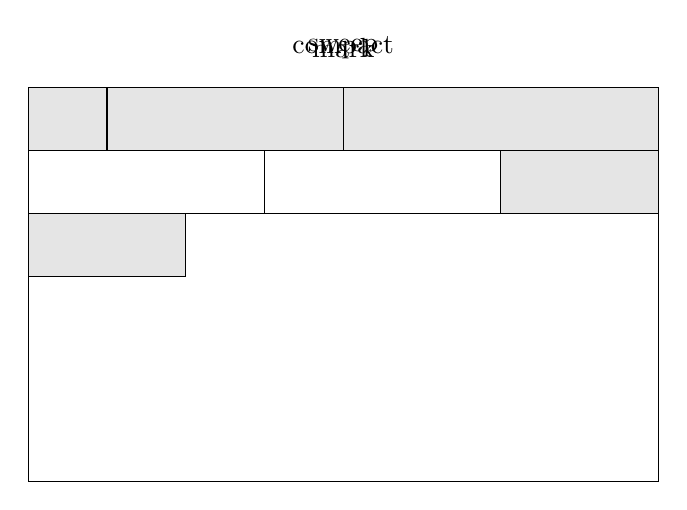
\begin{tikzpicture}[ampersand replacement=\&]
      \draw (0,0) rectangle (8,5);
      \draw [fill=light-grey] (0,4.2) rectangle (1,5);
      \visible<1-2>{\draw [alt=<2>{fill=Thistle}{fill=light-grey}] (1,4.2) rectangle (4,5);};
      \visible<1-3>{\draw [fill=light-grey] (4,4.2) rectangle (7,5);}
      \visible<1-2>{\draw [alt=<2>{fill=Thistle}{fill=light-grey}] (7,4.2) rectangle (8,5);}
      \visible<1-2>{\draw [alt=<2>{fill=Thistle}{fill=light-grey}] (0,3.4) rectangle (3,4.2);}
      \visible<1-2>{\draw [alt=<2>{fill=Thistle}{fill=light-grey}] (3,3.4) rectangle (6,4.2);}
      \visible<1-3>{\draw [fill=light-grey] (6,3.4) rectangle (8,4.2);}
      \visible<1-3>{\draw [fill=light-grey] (0,2.6) rectangle (2,3.4);}
      \visible<4>{\draw [fill=light-grey] (1,4.2) rectangle (4,5);}
      \visible<4>{\draw [fill=light-grey] (4,4.2) rectangle (8,5);}
      \visible<2>{\node [align=center] at (4,5.5) {mark};}
      \visible<3>{\node [align=center] at (4,5.5) {sweep};}
      \visible<4>{\node [align=center] at (4,5.5) {compact};}
    \end{tikzpicture}
  \end{center}
  \note<1>[item]{Let's take a look at how garbage collection is performed by the .NET runtime.}
  \note<1>[item]{We'll take the allocations shown as an example of the different steps in the process.}
  \note<1>[item]{This is a simplification, and the real runtime has a number of differences to this, but it is a close enough model that works when debugging memory issues.}
  \note<2>[item]{The first step is to find all those allocations (normally objects or arrays) that aren't being used any more.}
  \note<2>[item]{These objects are \emph{marked} for deletion in this stage.}
  \note<3>[item]{There are two options for the second stage, depending on whether we want a quick garbage collection or a full garbage collection.}
  \note<3>[item]{The quickest option is to \emph{sweep}, which means to deallocate all those allocations that were marked in the first stage.}
  \note<3>[item]{This is quite quick to perform, but has a disadvantage that the memory is now fragmented, as you can see. This makes it harder to perform other allocations in the future, because they need to fit in the gaps left by the sweep.}
  \note<4>[item]{The alternative to sweep is to \emph{compact}. This is where we shuffle all the used objects down so there aren't any gaps. This involves updating all references to those objects which takes a long time.}
  \note<4>[item]{Compacting is slow, but leaves the memory unfragmented. In practice .NET does a mix of mark-sweep and mark-compact depending on the current memory state.}
\end{frame}

\begin{frame}[fragile]{Garbage collection}
  \begin{center}
    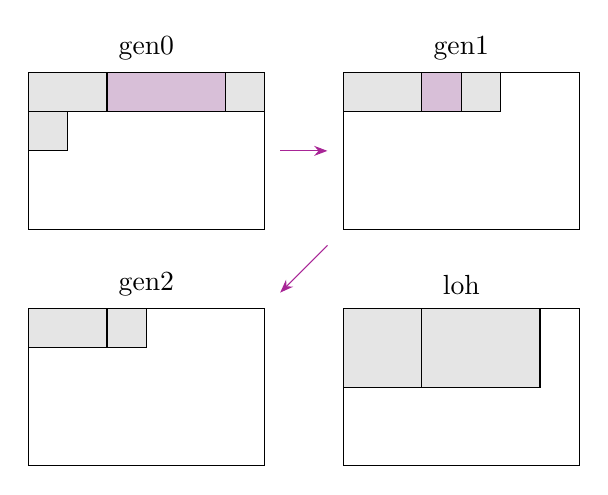
\begin{tikzpicture}[ampersand replacement=\&]
      \visible<2->{\node [align=center] at (1.5,5.3) {gen0};}
      \draw (0,3) rectangle (3,5);
      \visible<1>{
        \draw [fill=light-grey] (0,4.5) rectangle (1,5);
        \draw [fill=Thistle] (1,4.5) rectangle (2.5,5);
        \draw [fill=light-grey] (2.5,4.5) rectangle (3,5);
        \draw [fill=light-grey] (0,4) rectangle (0.5,4.5);
      }
      \visible<2>{
        \draw [draw=Mulberry,-{Stealth}] (3.2,4) -- (3.8,4);
        \draw [fill=light-grey] (4,4.5) rectangle (5,5);
        \draw [fill=Thistle] (5,4.5) rectangle (5.5,5);
        \draw [fill=light-grey] (5.5,4.5) rectangle (6,5);
      }
      \visible<2->{
        \node [align=center] at (5.5,5.3) {gen1};
        \draw (4,3) rectangle (7,5);
      }
      \visible<3>{\draw [draw=Mulberry,-{Stealth}] (3.8,2.8) -- (3.2,2.2);}
      \visible<3->{
        \node [align=center] at (1.5,2.3) {gen2};
        \draw (0,0) rectangle (3,2);
        \draw [fill=light-grey] (0,1.5) rectangle (1,2);
        \draw [fill=light-grey] (1,1.5) rectangle (1.5,2);
      }
      \visible<4->{
        \node [align=center] at (5.5,2.3) {loh};
        \draw (4,0) rectangle (7,2);
        \draw [fill=light-grey] (4,1) rectangle (5,2);
        \draw [fill=light-grey] (5,1) rectangle (6.5,2);
      }
    \end{tikzpicture}
  \end{center}
  \note<1>[item]{There's one other aspect of garbage collection that we should look called \emph{generations}. At first this doesn't seem particularly important, but the more you learn about garbage collection the more relevant generations become.}
  \note<1>[item]{Let's take the example shown here where there's a single item marked for collecting during garbage collection. For now let's not worry whether we are using mark-sweep or mark-compact.}
  \note<2>[item]{When the garbage collector runs, any objects in \texttt{gen0} (generation 0) that aren't garbage collected are `moved' to \texttt{gen1}.}
  \note<2>[item]{Don't worry for now about whether these are separate or shared parts of physical memory---the reality is somewhat complicated---but we can treat them as if they are physically separate.}
  \note<2>[item]{\texttt{gen0} and \texttt{gen1} have a certain amount of space in them (they have their own quotas).}
  \note<3>[item]{When garbage collection runs again, anything in \texttt{gen1} that is still alive is moved to \texttt{gen2} as you might expect. This also has its own quota.}
  \note<3>[item]{Can you guess what happens if we run garbage collection again?}
  \note<4>[item]{Actually, \texttt{gen2} is the last storage, and is used for anything that's long-lived.}
  \note<4>[item]{Things that go into \texttt{gen2} are either deleted or stay in \texttt{gen2}.}
  \note<4>[item]{To complicate matters slightly, you will see there is also a separate area marked \texttt{loh} which refers to the `large object heap'. This stores all large objects allocated, regardless of how many generations they have been around for.}
\end{frame}

\begin{frame}[fragile]{GC roots}
  \begin{center}
    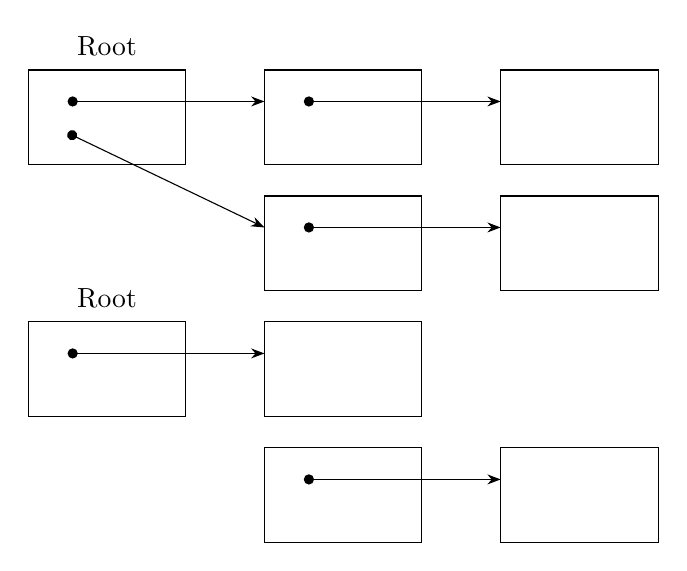
\begin{tikzpicture}[ampersand replacement=\&]
      \node [align=center] at (1,6.5) {Root};
      \draw [alt=<2->{fill=light-grey}{}] (0,5) rectangle (2,6.2);
      \draw [Circle-Stealth] (0.5,5.8) -- (3,5.8);
      \draw [alt=<3->{fill=light-grey}{}] (3,5) rectangle (5,6.2);
      \draw [Circle-Stealth] (3.5,5.8) -- (6,5.8);
      \draw [alt=<3->{fill=light-grey}{}] (6,5) rectangle (8,6.2);
      \draw [Circle-Stealth] (0.5,5.4) -- (3,4.2);
      \draw [alt=<3->{fill=light-grey}{}] (3,3.4) rectangle (5,4.6);
      \draw [Circle-Stealth] (3.5,4.2) -- (6,4.2);
      \draw [alt=<3->{fill=light-grey}{}] (6,3.4) rectangle (8,4.6);
      \node [align=center] at (1,3.3) {Root};
      \draw [alt=<2->{fill=light-grey}{}] (0,1.8) rectangle (2,3);
      \draw [Circle-Stealth] (0.5,2.6) -- (3,2.6);
      \draw [alt=<3->{fill=light-grey}{}] (3,1.8) rectangle (5,3);
      \invisible<5>{
        \draw [alt=<4->{fill=Thistle}{}] (3,0.2) rectangle (5,1.4);
        \draw [Circle-Stealth] (3.5,1) -- (6,1);
        \draw [alt=<4->{fill=Thistle}{}] (6,0.2) rectangle (8,1.4);
      }
    \end{tikzpicture}
  \end{center}
  \note<1>[item]{The last bit of theory that's worth looking at is how the `mark' algorithm decides whether an object should be deallocated.}
  \note<1>[item]{Let's imagine we have some objects that refer to other objects (that is, they have a reference in an instance variable to that object). We don't have any cycles here, but it doesn't significantly changes things if we did.}
  \note<1>[item]{Some of these objects are `root' objects. These are special objects that the garbage collector knows you definitely want. Mostly they are objects referenced in the stack somewhere, or by a static variable.}
  \note<2>[item]{The garbage collector knows that you need the root objects, so it knows these shouldn't be marked.}
  \note<3>[item]{It can also work out that you need any objects that these root objects refer to.}
  \note<3>[item]{This forms a graph, and the garbage collector just needs to explore all nodes in the graph to find all nodes that are still needed.}
  \note<4>[item]{Finally, the mark algorithm can mark anything that hasn't been identified as being needed.}
  \note<5>[item]{And then these marked objects can be deallocated in the sweep or compact stage.}
\end{frame}

\begin{frame}[standout]
\end{frame}
\note[itemize]
{
  \item First show code for \texttt{SimpleLeaker} and point out in \texttt{dotMemory} the memory allocations over time and in the generations (including large object heap).
  \item After the large object heap allocation force a garbage collect and take a snapshot. Then after the two subsequent clears force a garbage collect. Point out retention in stack storage.
  \item Demonstrate overview, dominators, similar retention (showing GC roots).
  \item Next show \texttt{CodeRunner}. Show the dominators point to the statement cache. Open objects retained by that retention path and show the similar retention path.
  \item Point out that we should try and work out why \texttt{OracleInternal.Common.StatementCache} is retaining all the \texttt{CachedStatement} instances.
}

\section{Why?}
\note[itemize]
{
  \item Now that we've found where the memory leak is, we need to understand why the Oracle library is holding on to all the statements.
  \item To do that we'll first review how compilation happens in .NET, so we can see how we can reverse this process in order to understand third-party code we don't have the source code for.
  \item This process is called `reverse engineering'.
  \item Again, we'll see this process for our simple application (that we do have the source for) before looking at the Oracle library used by \texttt{CodeRunner}.
}

\begin{frame}[fragile]{Common Language Runtime}
  \begin{center}
    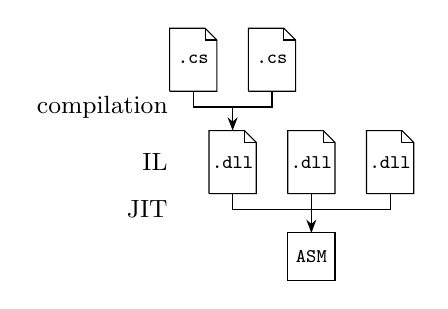
\begin{tikzpicture}[ampersand replacement=\&]
      \draw (0,6) pic {csfile};
      \draw (1,6) pic {csfile};
      \draw (0.3,6) -- (0.3,5.8) -- (1.3,5.8) -- (1.3,6);
      \draw [-{Stealth}] (0.8,5.8) -- (0.8,5.5);
      \draw (0.5,4.7) pic {dllfile};
      \node [left] at (0.1,5.8) {\small compilation};
      \visible<1>{\node [left] at (0.1,5.1) {\small IL};}
      \visible<2>{
        \draw (1.5,4.7) pic {dllfile};
        \draw (2.5,4.7) pic {dllfile};
        \draw (0.8,4.7) -- (0.8,4.5) -- (2.8,4.5) -- (2.8,4.7);
        \draw (1.8,4.7) -- (1.8,4.5);
        \draw [-{Stealth}] (1.8,4.5) -- (1.8,4.2);
        \draw (1.5,3.6) pic {asm};
        \node [left] at (0.1,4.5) {\small JIT};
      }
    \end{tikzpicture}
  \end{center}
  \note<1>[item]{In C\#, the compiler will take multiple source files that are part of a project, and compile them into something called an assembly. In recent versions of .NET, this always has the extension \texttt{.dll}.}
  \note<1>[item]{This collection of compiled code is in a platform-independent format called \emph{intermediate language}. In fact, the compiled code still retains much of the original structure such as classes and variable names even.}
  \note<1>[item]{The purpose of the intermediate language is to make the code cross-platform so it can be run on a different operating system, and hardware. The language is higher-level than a CPU, but lower level than languages like C\#.}
  \note<2>[item]{At runtime, all the different assemblies that are needed to run the program are collected together by the runtime and compiled into machine code for the particular hardware platform.}
  \note<2>[item]{This second compilation step is normally done only when the code in needed. So some functions will be compiled to machine code, but other functions will be left until they are needed. This process is called \emph{just-in-time compilation}.}
  \note<2>[item]{The key to all this process is that we can take any file in the intermediate language (IL) and attempt to reverse the compilation process. Because much of the structure of the original code is retained in IL, this decompilation step is quite accurate and readable.}
\end{frame}

\begin{frame}[standout]
\end{frame}
\note[itemize]
{
  \item Show how \texttt{dotPeak} works on \texttt{SimpleLeaker}. Demonstrate the source view when source is available, the decompiled sources, and the IL view.
  \item Next open up the \texttt{Oracle.ManagedDataAccess.dll} and find \texttt{OracleInternal.Common.StatementCache}.
  \item Find references to \texttt{m\_maxCacheSize} and then the constructor for \texttt{StatementCache}. Then see where \texttt{recommendedScs} comes from and how it is set.
  \item In particular pay attention to the last reference in \texttt{OraclePoolManager.Initialize} and how the \texttt{ProviderConfig} gets the value for \texttt{MaxStatementCacheSize}.
}

\begin{frame}[fragile]{Case study}
  The `bug' is `fixed' with
  \begin{verbatim}
    MaxStatementCacheSize = 50
  \end{verbatim}
\end{frame}
\note[itemize]
{
  \item Setting the \texttt{MaxStatementCacheSize} to a lower value reduced the statement cache without making a significant difference to the performance of database queries since the statements weren't able to be reused in most cases.
  \item The bug was ultimately fixed by a simple database connection configuration change.
  \item One of the differences between the old version and the new was an update to the Oracle .NET package. But that by itself wouldn't easily point to what the solution was---memory dump analysis and reverse engineering are useful skills to help understand difficult bugs.
}

\section{How?}
\note{I'll finish with a few suggestions on additional tools that can help as well as where to go to learn more about all of this.}

\begin{frame}[fragile]{Tools}
  Memory analysis
  \begin{itemize}
    \item \texttt{dotMemory}
    \item \texttt{dotnet-dump}
    \item \texttt{dotnet-counters}
    \item \texttt{PerfView}
  \end{itemize}

  Decompilers
  \begin{itemize}
    \item \texttt{dotPeak}
    \item \texttt{ildasm}
    \item \texttt{ILSpy}
    \item \texttt{dnSpy}
  \end{itemize}
\end{frame}
\note[itemize]
{
  \item \texttt{dotnet-counters} gives live summary statistics for the memory management.
  \item \texttt{dotnet-dump} allows you to collect dumps and analyse them similarly to \texttt{dotMemory} but using a command line and with more detail.
  \item \texttt{PerfView} is a tool from Microsoft that does everything \texttt{dotMemory} can do and a lot more. It is probably the most complete performance analysis tool available (particularly for .NET). It is unfortunately not widely used, in part because it has a steep learning curve. It does have excellent documentation, however.
  \item \texttt{ildasm} is the original disassembler for the .NET intermediate language. It is a command-line tool that is low frills and mainly useful for batch processing.
  \item \texttt{ILSpy} is similar to \texttt{dotPeak} but free and open source.
  \item \texttt{dnSpy} can also debug processes which can be useful to see the intermediate language during debugging. However, it isn't really an intermediate language debugger as it doesn't give information that would be useful (such as the IL stack state)---these don't seem to exist, unfortunately.
}

\begin{frame}[fragile]{Tools}
  Debuggers
  \begin{itemize}
    \item \texttt{Visual Studio} debugger
    \item \texttt{dnSpy}
    \item \texttt{WinDbg}
  \end{itemize}

  Honourable mention
  \begin{itemize}
    \item \texttt{SysInternals}
  \end{itemize}
\end{frame}
\note[itemize]
{
  \item \texttt{WinDbg} is \emph{the} Windows debugger. For .NET it combines the power of a usual debugger with the memory information from \texttt{dotnet-dump}, but live. It shares the same tools as \texttt{dotnet-dump} using what is called \texttt{SOS}.
  \item \texttt{SysInternals} is worth mentioning because it is a collection of tools that are immensely useful for debugging all kinds of issues on Windows. If you don't already know about these, you should learn.
}

\begin{frame}[fragile]{Guides}
  \printbibliography[heading=none]
\end{frame}
\note[itemize]
{
  \item \autocite{CsiDotNet} is a presentation that goes over more ground that this talk but in a very accessible way. It was part of a JetBrains .NET conference a few years ago.
  \item \autocite{MemDoc} contains a wealth of information from the .NET GC architect. In particular there's a how-to guide on memory performance analysis that goes into an enormous amount of information.
}

\end{document}
